
\documentclass[a4paper,12pt]{article}
\usepackage[slovene]{babel}
\usepackage[utf8]{inputenc}
\usepackage[T1]{fontenc}
\usepackage{lmodern}
\usepackage{float}
\usepackage{url}
\usepackage[]{amsmath}
\usepackage[]{amsthm}
\usepackage[]{graphicx}
\usepackage{amssymb}

\newcommand{\pojem}[1]{\underline{\textsc{#1}}}

\theoremstyle{definition}
\newtheorem{definicija}{Definicija}

\theoremstyle{plain}
\newtheorem{izrek}{Izrek}

\newenvironment{dokaz}{\begin{proof}[Dokaz izreka]}{\end{proof}}

\setlength\parindent{0pt}

\begin{document}

\thispagestyle{empty}
\begin{center}
\begin{minipage}{0.75\linewidth}
    \centering
    {\Large Univerza v Ljubljani \\ Fakulteta za matematiko in fiziko}
    \\
    \vspace{7cm}

    {\uppercase{\Large \textbf{Scheduling triangles}}} \\ Finančni praktikum \\
    \vspace{5cm}

    Avtorja:\\
    { Blaž Arh, Matic Matušek}
    \vspace{5cm}

    {\Large Ljubljana, 2022}
\end{minipage}
\end{center}


\newpage
\tableofcontents
\newpage



\section{Uvod}
\subsection{Navodilo naloge}

Imamo $n$ pravokotnih enakokrakih trikotnikov, ki so določeni z dolžino kraka $d_i$ za $i=1,2,...,n$  in pravim kotom med krakoma.
Trikotnike postavimo, z nogo na $x$-os, na sledeči način.
\begin{center}
   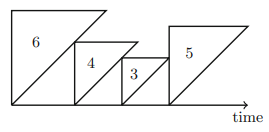
\includegraphics[width=8cm, height=4cm]{primer_trikotnikov.png} 
\end{center}

Trikotniki morajo biti postavljeni tako, da je hipotenuza trikotnika naraščajoča glede na $x$-os, natančneje naklon hipotenuze je enak 1. \\
Želimo si trikotnike postaviti tako, da je dolžina teh trikotnikov najkrajša. Trikotniki se med seboj ne smejo prekrivati,
prav tako pa mora biti krak noge pravokoten na $x$-os.

\subsection{Uporabnost}
Pomembno je, da znamo ta matematični problem interpretirati v praksi. \\
Torej:
\begin{itemize}
    \item pravokotni enakokraki trikotniki $=$ opravila,
    \item dolžina kraka $=$ pomembnost opravila.
\end{itemize}

Želimo si sestaviti urnik iz $n$ opravil. Naj bo $d_i$ pomembnost $i$-tega opravila. Naš cilj je sestaviti čim krajši urnik. Želimo, da se pomembnejša opravila izvedejo, v primeru zakasnitve le teh pa lahko manj pomembna opravila izpustimo.
Večji kot je trikotnik, bolj pomembno je opravilo. Kot je razvidno iz zgornje slike, lahko opravila z manjšo pomembnostjo vstavimo pod opravila z večjo pomembnostjo. To pomeni, da manjše trikotnike vstavljamo pod večje. Torej, če pride do zakasnitve
pomembnejšega opravila (večjega trikotnika), manj pomembno opravilo  izpustimo (manjši trikotnik).


\section{Reševanje problema s pomočjo različnih algoritmov}
Reševanja najinega problema sva se lotila s pomočjo treh algoritmov:
\begin{itemize}
    \item bruteforce algoritem
    \item Greedy algoritem
    \item algoritem, ki s pomočjo celoštevilškega lineranega programiranja išče optimalno rešitev.
\end{itemize}

\subsection{Brute force algoritem}
\subsubsection{Opis algoritma}
Algoritem iz n trikotnikov sestavi vse možne permutacije in izračuna njihovo dolžino. Nato 
pa izbire prvo permutacijo na katero je naletel, ki je imela minimalno dolžino.
\subsubsection{Psevdokoda}
\begin{verbatim}
    1.    Vhod: trikotniki
    2.    n = length(trikotniki)
    3.    dolzina_urnika = []
        perutacije = permutations( [0, 1, ..., n-1] )
        for i in permutacije
            for j in 0:(n-1)
                trikotnik["vrstni_red"][j] = permutacija[j]
            dolzina_urnika.append( dolzina(trikotniki) )
        index = dolzina_urnika.index( min(dolzina_urnika) )
        for i in 0:(n-1)
            trikotniki[i]["vrstni red"] = permutacije[index][i]
        Izhod: trikotniki

\end{verbatim}




\subsection{Greedy algoritem}
\subsubsection{Opis algoritma}
Greedy algoritem je kateri koli algoritem, ki rešuje problem tako, da na vsakem koraku naredi lokalno optimalno izbiro.
Greedy algoritem najprej razvrsti trikotnike tako, da velja \newline
$d_1 \geq d_2 \geq d_3 \geq ... \geq d_n$. Prvi trikotnik razvrsti na $x=0$, kar ustvari prostor pod trikotnikom 1.
Nato vsak trikotnik $j=2,...,n$ postavi v največji možen prostor pod že postavljenimi trikotniki. Če je več enakih prostorov, izbere prvega povrsti.
Če ima izbrani prostor pod trikotnikom dolžino $l$ in se začne v času $x_i$, potem je trikotnik $j$ postavljen na mesto $x_j=x_i+d_j$. Če je $2d_j \ge l$,  potem se vsi trikotniki $k$, za katere je $x_k \ge x_j$ zamaknejo za $ 2d_j-l$, da se ne prekrivajo. Opisano 
dogajanje prikazuje spodnji primer($x=l, p_i = d_i $).
\begin{center}
    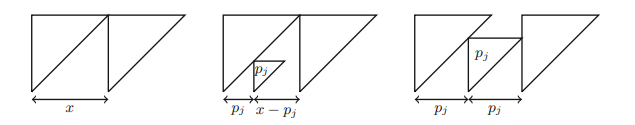
\includegraphics[width=13cm, height=3cm]{greedy.png} 
 \end{center}
Pri številnih problemih Greedy algoritem ne poišče optimalne rešitve, nič drugače ni pri našem problemu.
Na naslednji sliki prikažemo primer, ko Greedy ni optimalen. Greedy algoritem (desna slika) vrne dolzino 42 in ne vrne optimalne dolžine, ki je 40 (leva slika).
\begin{center}
    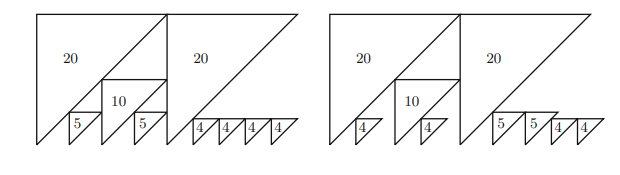
\includegraphics[width=10cm, height=3cm]{primer_neoptimalnosti_greedy.png} 
 \end{center}
Hitrost Greedy algoritma je polinomska. Da se pokazati, da je aproksimacijsko razmerje zgornje meje točnosti Greedy algoritma $1.5$ optimalnega časa. Torej, če je optimalni čas določenega primerna
$40$ časovnih enot, potem Greedy pokaže največ $60$ časovnih enot.

\subsubsection{Psevdokoda}
\begin{verbatim}
    Vhod: trikotniki
    n = length(trikotniki)
    trikotniki_lokalno = dict()
    for i in 0:(n-1)
        trikotniki_lokalno[i] = trikotniki[i]
        m = length(trikotniki_lokalno)
        lokalna_dolzina_urnika = []
        for j in 0:(m-1):
            trikotniki_lokalno[i]["vrstni_red"] = j
            *popravi_mesta_ostalim_trikotnikom
            lokalna_dolzina_urnika.append( dolzina_urnika(trikotniki_lokalno) )
        index = lokalna_dolzina_urnika.index( min(lokalna_dolzina_urnika) )
        trikotniki_lokalno[i]["vrstni_red"] = index
        *popravi_mesta_ostalim_trikotnikom
    Izhod: trikotniki_lokalno

\end{verbatim}


Tukaj opisat popravi\_mesta...

%\subsubsection{Predsatvitev rezultatov}

%\subsection{Clp}
%\subsubsection{Opis algoritma}
\subsubsection{Psevdokoda}
\begin{verbatim}
    Vhod: seznam_dolzin_trikotnikov
    T = sum(seznam_dolzin_trikotnikov)
    t = new_variable()
    s = new_variable()
    x = new_variable(binary = True)
    set_objective(t, maximization = False)
    for i, d in enumerate(seznam_dolzin_trikotnikov)
        add_constraint(s[i] >= 0)
        add_constraint(s[i] + d <= t)
        for j, e in enumerate(seznam_dolzin_trikotnikov[i+1:], i+1):
            m = min(d, e)
            add_constraint(x[i, j]+x[j, i] = 1)
            add_constraint(s[i] - s[j] >= m - T*x[j, i])
            add_constraint(s[j] - s[i] >= m - T*x[i, j])
    Izhod: seznam s
\end{verbatim}
v seznamu s so napisani položaji nog trikotnikov

\subsection{Generiranje podatkov}

\subsection{Predstavitev rezultatov}
\begin{verbatim}
    test = naredi_trikotnike(
                9,
                [ 
                44.513033703890834,
                18.613265453372076,
                27.04233495394404,
                29.803779538038164,
                38.01467639495788,
                43.53220098011497,
                13.90897209250403,
                26.415619884578483,
                49.01780933958118
                ]
            )
\end{verbatim}

seznam trikotnikov, ime algoritma, več optimalnih razporeditev 
število optimalnih rešitev 72. \\
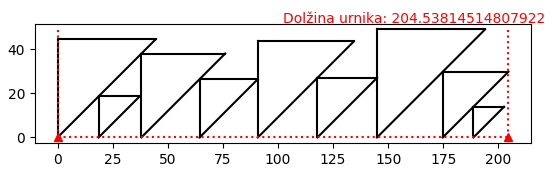
\includegraphics[]{sim_brut.png}
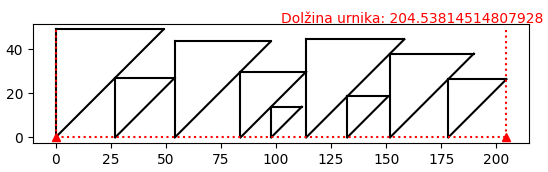
\includegraphics[]{sim_clp.png}
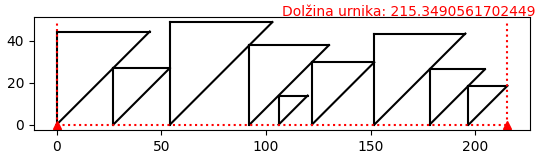
\includegraphics[]{sim_greedy.png}




\end{document}